% !TEX root = ../mainthesis.tex

\chapter[Flexural strength and flaw distributions of \ce{SrFe_{0.2}Co_{0.4}Mo_{0.4}O_{3}} based ceramic-supports for solid-oxide fuel cells at operating conditions]{Flexural strength and flaw distributions of\\ \ce{SrFe_{0.2}Co_{0.4}Mo_{0.4}O_{3}} based ceramic-supports for \\solid-oxide fuel cells at operating conditions}

\section{Introduction}
    This work characterizes the changes which occur in fracture toughness and flaw distributions of SFCM, SFCM-GDC \gls{asl}, and SFCM-GDC/GDC half-cells when exposed to oxidizing and reducing conditions up to \SI{600}{\celsius} by use of flexural testing and Weibull analysis.
    Additionally, electrical conductivity, thermogravimetric analysis, and thermal expansion are used to determine the causes for changes in mechanical properties under these conditions.

\section{Results and Discussion}
    \subsection{Redox Cycling Stability}
        SFCM has a high initial conductivity of \SI{35}{S\per\centi\meter} but decreases after 3 cycles to \SI{19}{S\per\centi\meter} and again at 9 cycles, shown in Figure \ref{fig:TGA}a.
        The addition of GDC to create a SFCM-GDC composite decreases the initial conductivity to \SI{15}{S\per\centi\meter}.
        At 4 cycles, SFCM-GDC decreases conductivity and stabilizes to \SI{8}{S\per\centi\meter} for 19 cycles.
        The addition of the GDC improved the redox cycling stability by providing a very stable, contiguous framework for the SFCM.\cite{Mogensen2000,Duncan2006,Bishop2009}

        Figure \ref{fig:TGA}b shows the mass loss of SFCM-GDC as it is reduced in 3\% humidified H\textsubscript{2}.
        For comparison, another popular anode material, nickel oxide GDC, is plotted along with it.
        The reduction of SFCM-GDC results in a less than 1\% reduction of mass from the formation of oxygen vacancies in the SFCM and GDC, and it reaches steady state in under two hours.
        NiO-GDC on the other hand loses a large amount of mass from the reduction and phase change of NiO to Ni metal, taking over 30 hours to reach steady state.

        \begin{figure}
          \includegraphics[width=0.6\textwidth]{CycleConductivity.jpg}
          \includegraphics[width=0.6\textwidth]{TGA.jpg}
          \caption{a) DC conductivity of SFCM and SFCM-GDC after cycling at \SI{650}{\celsius} between 10\% H\textsubscript{2} in N\textsubscript{2} and air. b) Mass loss of SFCM-GDC and NiO-GDC during reduction in 3\% H\textsubscript{2}/3\% H\textsubscript{2}O in N\textsubscript{2} at \SI{650}{\celsius}.}
          \label{fig:TGA}
        \end{figure}

        Further cycling of SFCM in the \gls{tga} was performed and results are given in Figure \ref{fig:Cycled}, with \ref{fig:Cycled}a showing the mass loss of SFCM with time as it is cycled between air and hydrogen, and \ref{fig:Cycled}b being a summary of the total mass changes that occur with each cycle.
        With each cycle, less than 1\% total mass change is observed.
        Reduction occurs over a time period of five hours while oxidation happens at a faster rate, approximately one hour.
        Fitting the reduction and oxidation to exponential functions gives a biexponential with decay rates of 0.438 and 27.89 for reduction and an oxidation rate of 2.90.
        Previous experiments have shown that SFCM generates an impurity phase of \ce{Sr_2Co_{1.2}Mo_{0.8}O_6} under ambient and oxidizing conditions.\cite{Stanley2018}
        This impurity phase does not contribute to the gain or loss of oxygen as seen in the TGA.
        \ce{Sr_2Co_{1.2}Mo_{0.8}O_6} has a cubic structure compared to SFCM's tetragonal structure, leading to additional stress and strain created by its generation impacting the mechanical and electrical properties between oxidizing and reducing environments.

        \begin{figure}
          \includegraphics[width=0.6\textwidth]{TGACycle.jpg}
          \includegraphics[width=0.6\textwidth]{CycleSummary.jpg}
          \caption{Mass changes of SFCM during cycling between 21\% O\textsubscript{2} and 3\% H\textsubscript{2}/3\% H\textsubscript{2}O in N\textsubscript{2} at \SI{600}{\celsius}. Each exposure was 5 hours. a) Percent mass change with time as the gas is switched back and forth. b) Summary of maximum and minimum changes with each cycle.}
          \label{fig:Cycled}
        \end{figure}

    \subsection{Fracture Toughness}
        Fracture toughness was found to be \SI[separate-uncertainty = true]{0.124 +- 0.023}{\mega\pascal\sqrt{m}} at room temperature, increasing with temperature up to \SI{600}{\celsius}, as shown in Figure \ref{fig:Kic}a.
        From room temperature to \SI{500}{\celsius}, the rate of increase in K\textsubscript{Ic} is low at \SI{4.3e-5}{\mega\pascal\sqrt{m}\per\celsius}.
        From \SI{500}{\celsius} to \SI{600}{\celsius}, the fracture toughness increases by 90\%.
        The increase in fracture toughness is a result of the thermal expansion of the material.
        During process of creating the bar, the sample was cooled from \SI{1340}{\celsius} to room temperature.
        This cooling and associated contraction induces stresses in the bar sample, which combine with the stresses added during testing to fracture the sample.
        As the sample is heated, the residual stresses are relaxed, increasing the amount of stress which must be applied externally to cause the bar to fracture.
        Any change in fracture toughness due to the weakening of bonds is masked by this effect.
        The increase in fracture toughness from \SI{500}{\celsius} to \SI{600}{\celsius} matches the temperature where the rate of thermal expansion also increases, as shown in Figure \ref{fig:Kic}b.

        Figure \ref{fig:Kic}b also presents the thermal expansion of GDC and a SFCM-GDC composite.
        At temperatures below \SI{550}{\celsius}, the expansion of SFCM-GDC matches that of pure SFCM, greater than that of pure GDC.
        Above \SI{550}{\celsius}, the rate of expansion slows in comparison to SFCM and matches the rate of expansion for GDC.
        Thus, below \SI{550}{\celsius}, SFCM-GDC expands the same as SFCM and above \SI{550}{\celsius} it expands the same as GDC.
        We would then expect that SFCM-GDC composites have the same increase in fracture toughness as SFCM up to \SI{550}{\celsius} to due expansion and relaxation of intrinsic stresses, but not further increase the rate above \SI{500}{\celsius}, as SFCM does.

        \begin{figure}
          \includegraphics[width=0.6\textwidth]{Kic.jpg}
          \includegraphics[width=0.6\textwidth]{ThermalExpansion.jpg}
          \caption{a) Fracture toughness of SFCM from \SI{20}{\celsius} to \SI{600}{\celsius}. b) Thermal expansion of SFCM, GDC, and SFCM-GDC.}
          \label{fig:Kic}
        \end{figure}

    \subsection{Half-cell Strength of Anode-Supported SOFCs at Operating Conditions}
        Figure \ref{fig:InSituBox} gives box plots of the results of three point flexural testing of SFCM-GDC/GDC half-cells, and Table \ref{tab:halfcell} summaries the strengths.
        The circles on the right of \ref{fig:InSituBox} represent the results of a Student's t-test, to determine if the means of the different data sets are the same.
        The more the circles overlap the more similar the data sets are.
        In this case, there is no overlap between circles at the 95\% confidence interval, highlighting that the strengths tested at each condition are unique from each other.

        At ambient conditions the strength of the half-cells was measured to be \SI{57.7}{\mega\pascal}.
        Upon heating, the strength increases to \SI{74.2}{\mega\pascal}.
        This result correlates with the increase in fracture toughness discussed earlier, which is expected based on Equation \ref{eq:strength}.
        Another contributing factor to the increase in strength is the effect thermal expansion has on pre-existing cracks and flaws.
        Any expansion of the material helps push closed a surface crack which would lead to failure, decreasing its size and increasing the stress that would be required to cause that crack to open and propagate.

        Upon reduction of the half-cell at \SI{600}{\celsius}, the fracture strength decreases below that of the ambient strength to \SI{39.9}{\mega\pascal}.
        During this transition to reducing conditions, the impurity phase reduces back into SFCM, causing a decrease in mechanical properties from the change in lattice parameters.
        Additionally, bulk mechanical properties have changed as SFCM becomes pure phase, oxygen vacancies are generated and B-site transition metals are reduced.

        \begin{figure}[p]
          \includegraphics[width=\textwidth]{halfcellstrength.png}
          \caption{Flexural strengths of half-cell coupons made from SFCM-GDC anode with GDC electrolyte tested at \SI{20}{\celsius} in air, \SI{600}{\celsius} in air, and \SI{600}{\celsius} in 5\% H\textsubscript{2}.}
          \label{fig:InSituBox}
        \end{figure}

        \begin{table}
            \centering
            \caption{Summary of strengths for SFCM-GDC/GDC half-cells at different environments}
            \label{tab:halfcell}
            \begin{tabular}{lllll}
            \begin{tabular}[c]{@{}l@{}}Temperature\\(\SI{}{\celsius})\end{tabular} & Atmosphere & Number & \begin{tabular}[c]{@{}l@{}}Mean\\(MPa)\end{tabular} & \begin{tabular}[c]{@{}l@{}}Std Dev\\(MPa)\end{tabular}  \\
            \hline
            20                                                       & Air        & 17      & 57.7                                                & 6.71                                                    \\
            600                                                      & Air        & 5      & 74.2                                                & 2.98                                                    \\
            600                                                      & 5\% H2     & 14      & 39.9                                                & 5.89
            \end{tabular}
        \end{table}

        Weibull analysis was performed to compare the distribution of flaws between the ambient tested half-cells and the in-situ reduced half-cells.
        Figure \ref{fig:halfcellweibull} displays the fitting of Weibull distributions to the flexural strength of half-cell coupons tested at ambient conditions and during reduction at \SI{600}{\celsius}.
        Table \ref{tab:InSituWeibull} summarizes the fitting parameter for the Weibull modulus with 95\% confidence intervals using the maximum-likelihood method.
        Between the two conditions, there is an appreciable change in the Weibull modulus of the two samples.
        The Weibull modulus increases decreases from 10.4 at ambient conditions to 7.29 when at reducing conditions.
        This change in Weibull modulus is the result of the reduction of SFCM impurities changing the bulk properties of the material combined with distribution of flaws  becoming wider, creating more variability between flaws.

        To confirm any changes in flaw distribution, fractography would need to be performed on every sample, identifying the flaw, but this is not possible due to the porous nature of the fracture surface which obscures the fracture origin.
        Scanning electron microscopy was performed on fracture surfaces and epoxy-filled  samples from each condition to look for any microstructural changes.
        Figure \ref{fig:InSituSEM} shows the epoxy-filled and polished samples with no discernible difference between samples.
        No difference is observed because the likely cause of failure, microcracks, would exist along grain boundaries and are obscured by the grain boundaries and pores.\cite{Danzer2008,Yu2007}

        \begin{figure}
          \includegraphics[width=0.75\textwidth]{insituweibull.png}
          \caption{Fitted Weibull distributions of SFCM-GDC/GDC half-cells at different environments, plotted linearly with 95\% confidence intervals shaded.}
          \label{fig:halfcellweibull}
        \end{figure}

        \begin{table}
            \centering
            \caption{Summary of Weibull fitting parameters (characteristic strength and Weibull modulus) for SFCM-GDC/GDC half-cells at different environments}
            \label{tab:InSituWeibull}
            \begin{tabular}{llrrrrrr}
            \begin{tabular}[c]{@{}l@{}}Temp.~\\(\SI{}{\celsius})\end{tabular} & Environment & \multicolumn{1}{l}{\begin{tabular}[c]{@{}l@{}}Cha.~\\Strength\\(\textalpha{}, \SI{}{\mega\pascal})\end{tabular}} & \multicolumn{1}{l}{\begin{tabular}[c]{@{}l@{}}\textalpha~\\Lower\\CI\end{tabular}}& \multicolumn{1}{l}{\begin{tabular}[c]{@{}l@{}}\textalpha~\\Upper\\CI\end{tabular}}& \multicolumn{1}{l}{\begin{tabular}[c]{@{}l@{}}Weibull~\\Modulus\\ (\textbeta)\end{tabular}}& \multicolumn{1}{l}{\begin{tabular}[c]{@{}l@{}}\textbeta~\\Lower\\CI\end{tabular}}& \multicolumn{1}{l}{\begin{tabular}[c]{@{}l@{}}\textbeta~\\Upper\\CI\end{tabular}}  \\
            \hline
            20                                                        & Air         & 60.6                                                                                           & 57.4& 63.6& 10.4& 6.89& 14.7                                                                              \\
            600                                                       & Hydrogen    & 42.5                                                                                           & 39.2& 45.8& 7.29& 4.79& 10.3
            \end{tabular}
        \end{table}

        \begin{figure}
          \includegraphics[width=0.55\textwidth]{RTFracture.jpg}
          \includegraphics[width=0.55\textwidth]{HTfracture.jpg}
          \includegraphics[width=0.55\textwidth]{ReduceFracture.jpg}
          \caption{Scanning electron microscope images of epoxy-filled and polished SFCM-GDC/GDC half-cell cross sections tested at a) \SI{20}{\celsius} in air, b) \SI{600}{\celsius} in air and c) \SI{600}{\celsius} in 5\% H\textsubscript{2}}
          \label{fig:InSituSEM}
        \end{figure}

    \subsection{Strength of Anode Support Layer After Redox Cycling}
        To understand how redox cycling as the result of long term use affects the strength of SFCM based SOFCs, SFCM-GDC \gls{asl} test coupons were cycled for 10 times between nitrogen and 10\% H\textsubscript{2} environments.
        Figure \ref{fig:cycledbox} shows the strength and modulus from the samples which were not cycled (0 cycles) and those cycled 10 times, tested using a four-point bend at ambient conditions.
        Table \ref{tab:cycledsummary} summaries the means and standard deviations of the test results.
        The overlapping Student's t circles in Figure \ref{fig:cycledbox}b demonstrate that cycling did not significantly change the elastic modulus of the samples, while the strength did significantly decrease.
        This is the result of changes in microstructural flaws, rather than the change of an intrinsic material property.

        \begin{figure}
          \includegraphics[width=5in]{cycledbox.png}
          \includegraphics[width=5in]{cycledmod.png}
          \caption{Results of four point bend test at ambient conditions of SFCM-GDC \gls{asl} with a) strength and b) modulus for samples before any cycling and after 10 redox cycles between 10\% H\textsubscript{2} and N\textsubscript{2}.}
          \label{fig:cycledbox}
        \end{figure}

        \begin{table}
            \centering
            \caption{Summary of Cycled SFCM-GDC \gls{asl} Mechanical Properties}
            \label{tab:cycledsummary}
            \begin{tabular}{llllll}
            \begin{tabular}[c]{@{}l@{}}Number~\\of Cycles\end{tabular} & Number &  \begin{tabular}[c]{@{}l@{}}Mean~\\Modulus~\\(GPa)\end{tabular}& \begin{tabular}[c]{@{}l@{}}Modulus\\Std Dev~\\(GPa)\end{tabular}& \begin{tabular}[c]{@{}l@{}}Mean\\Strength\\(MPa)\end{tabular} & \begin{tabular}[c]{@{}l@{}}Strength~\\Std Dev~\\(MPa)\end{tabular} \\
            \hline
            0                                                          & 14     & 24.5                                                          & 5.01& 34.3& 7.23                                                                                                                                                                                      \\
            10                                                         & 20     & 27.3                                                          & 3.60& 22.4& 4.94
            \end{tabular}
        \end{table}

        The strengths of the cycled and un-cycled cells were fitted to Weibull distributions to observe how flaw distributions changed with redox cycling.
        Figure \ref{fig:cycledweibull} presents the fitted data and distributions and Table \ref{tab:cycledweibull} summarizes the fit parameters of the Weibull modulus with 95\% confidence intervals.
        The Weibull moduli between the two data sets are very similar, indicating that the flaw distribution is the same between them.
        The decrease in characteristic strength is then due to the growth of flaws with cycling.
        SEM images in Figure \ref{fig:cycledSEM} are of a sample which had not been cycled (a) and one which had been cycled 10 times (b) after being epoxy-filled and polished.
        The sample which had been cycled 10 times has a greater number of pores at larger sizes compared to the un-cycled sample.
        This indicates that the finer microstructure of the pores is susceptible to changes during redox cycling due to chemical expansion, but the larger flaws which lead to complete cell failure do not change as the result of redox cycling.\cite{Waldbillig2005}

        \begin{figure}[p]
          \includegraphics[width=0.75\textwidth]{cycledweibull.png}
          \caption{Fitted Weibull distributions of SFCM-GDC \gls{asl} before any cycling and after 10 redox cycles between 10\% H\textsubscript{2} and N\textsubscript{2}, plotted linearly with 95\% confidence intervals shaded}
          \label{fig:cycledweibull}
        \end{figure}

        \begin{table}
        \centering
        \caption{Summary of Weibull Fit Parameters (characteristic strength and Weibull modulus) for Cycled SFCM-GDC \gls{asl}}
        \label{tab:cycledweibull}
        \begin{tabular}{lrrrrrr}
        \begin{tabular}[c]{@{}l@{}}Number\\of Cycles\end{tabular} & \multicolumn{1}{l}{\begin{tabular}[c]{@{}l@{}}Char.~\\Strength~\\(\textalpha{}, \SI{}{\mega\pascal})\end{tabular}} & \multicolumn{1}{l}{\begin{tabular}[c]{@{}l@{}}\textalpha{}~\\CI Lower\end{tabular}} & \multicolumn{1}{l}{\begin{tabular}[c]{@{}l@{}}\textalpha{}~\\CI Upper\end{tabular}}& \multicolumn{1}{l}{\begin{tabular}[c]{@{}l@{}}Weibull~\\Modulus~\\(\textbeta{})\end{tabular}}& \multicolumn{1}{l}{\begin{tabular}[c]{@{}l@{}}\textbeta{}~\\CI Lower\end{tabular}}& \multicolumn{1}{l}{\begin{tabular}[c]{@{}l@{}}\textbeta{}~\\CI Upper\end{tabular}}  \\
        \hline
        0                                                         & 37.1                                                                                    & 33.7                                                                     & 40.8& 5.75& 4.06& 9.85                                                                                   \\
        10                                                        & 24.3                                                                                    & 22.3                                                                     & 26.5& 5.39& 4.00& 8.28
        \end{tabular}
        \end{table}

        \begin{figure}
          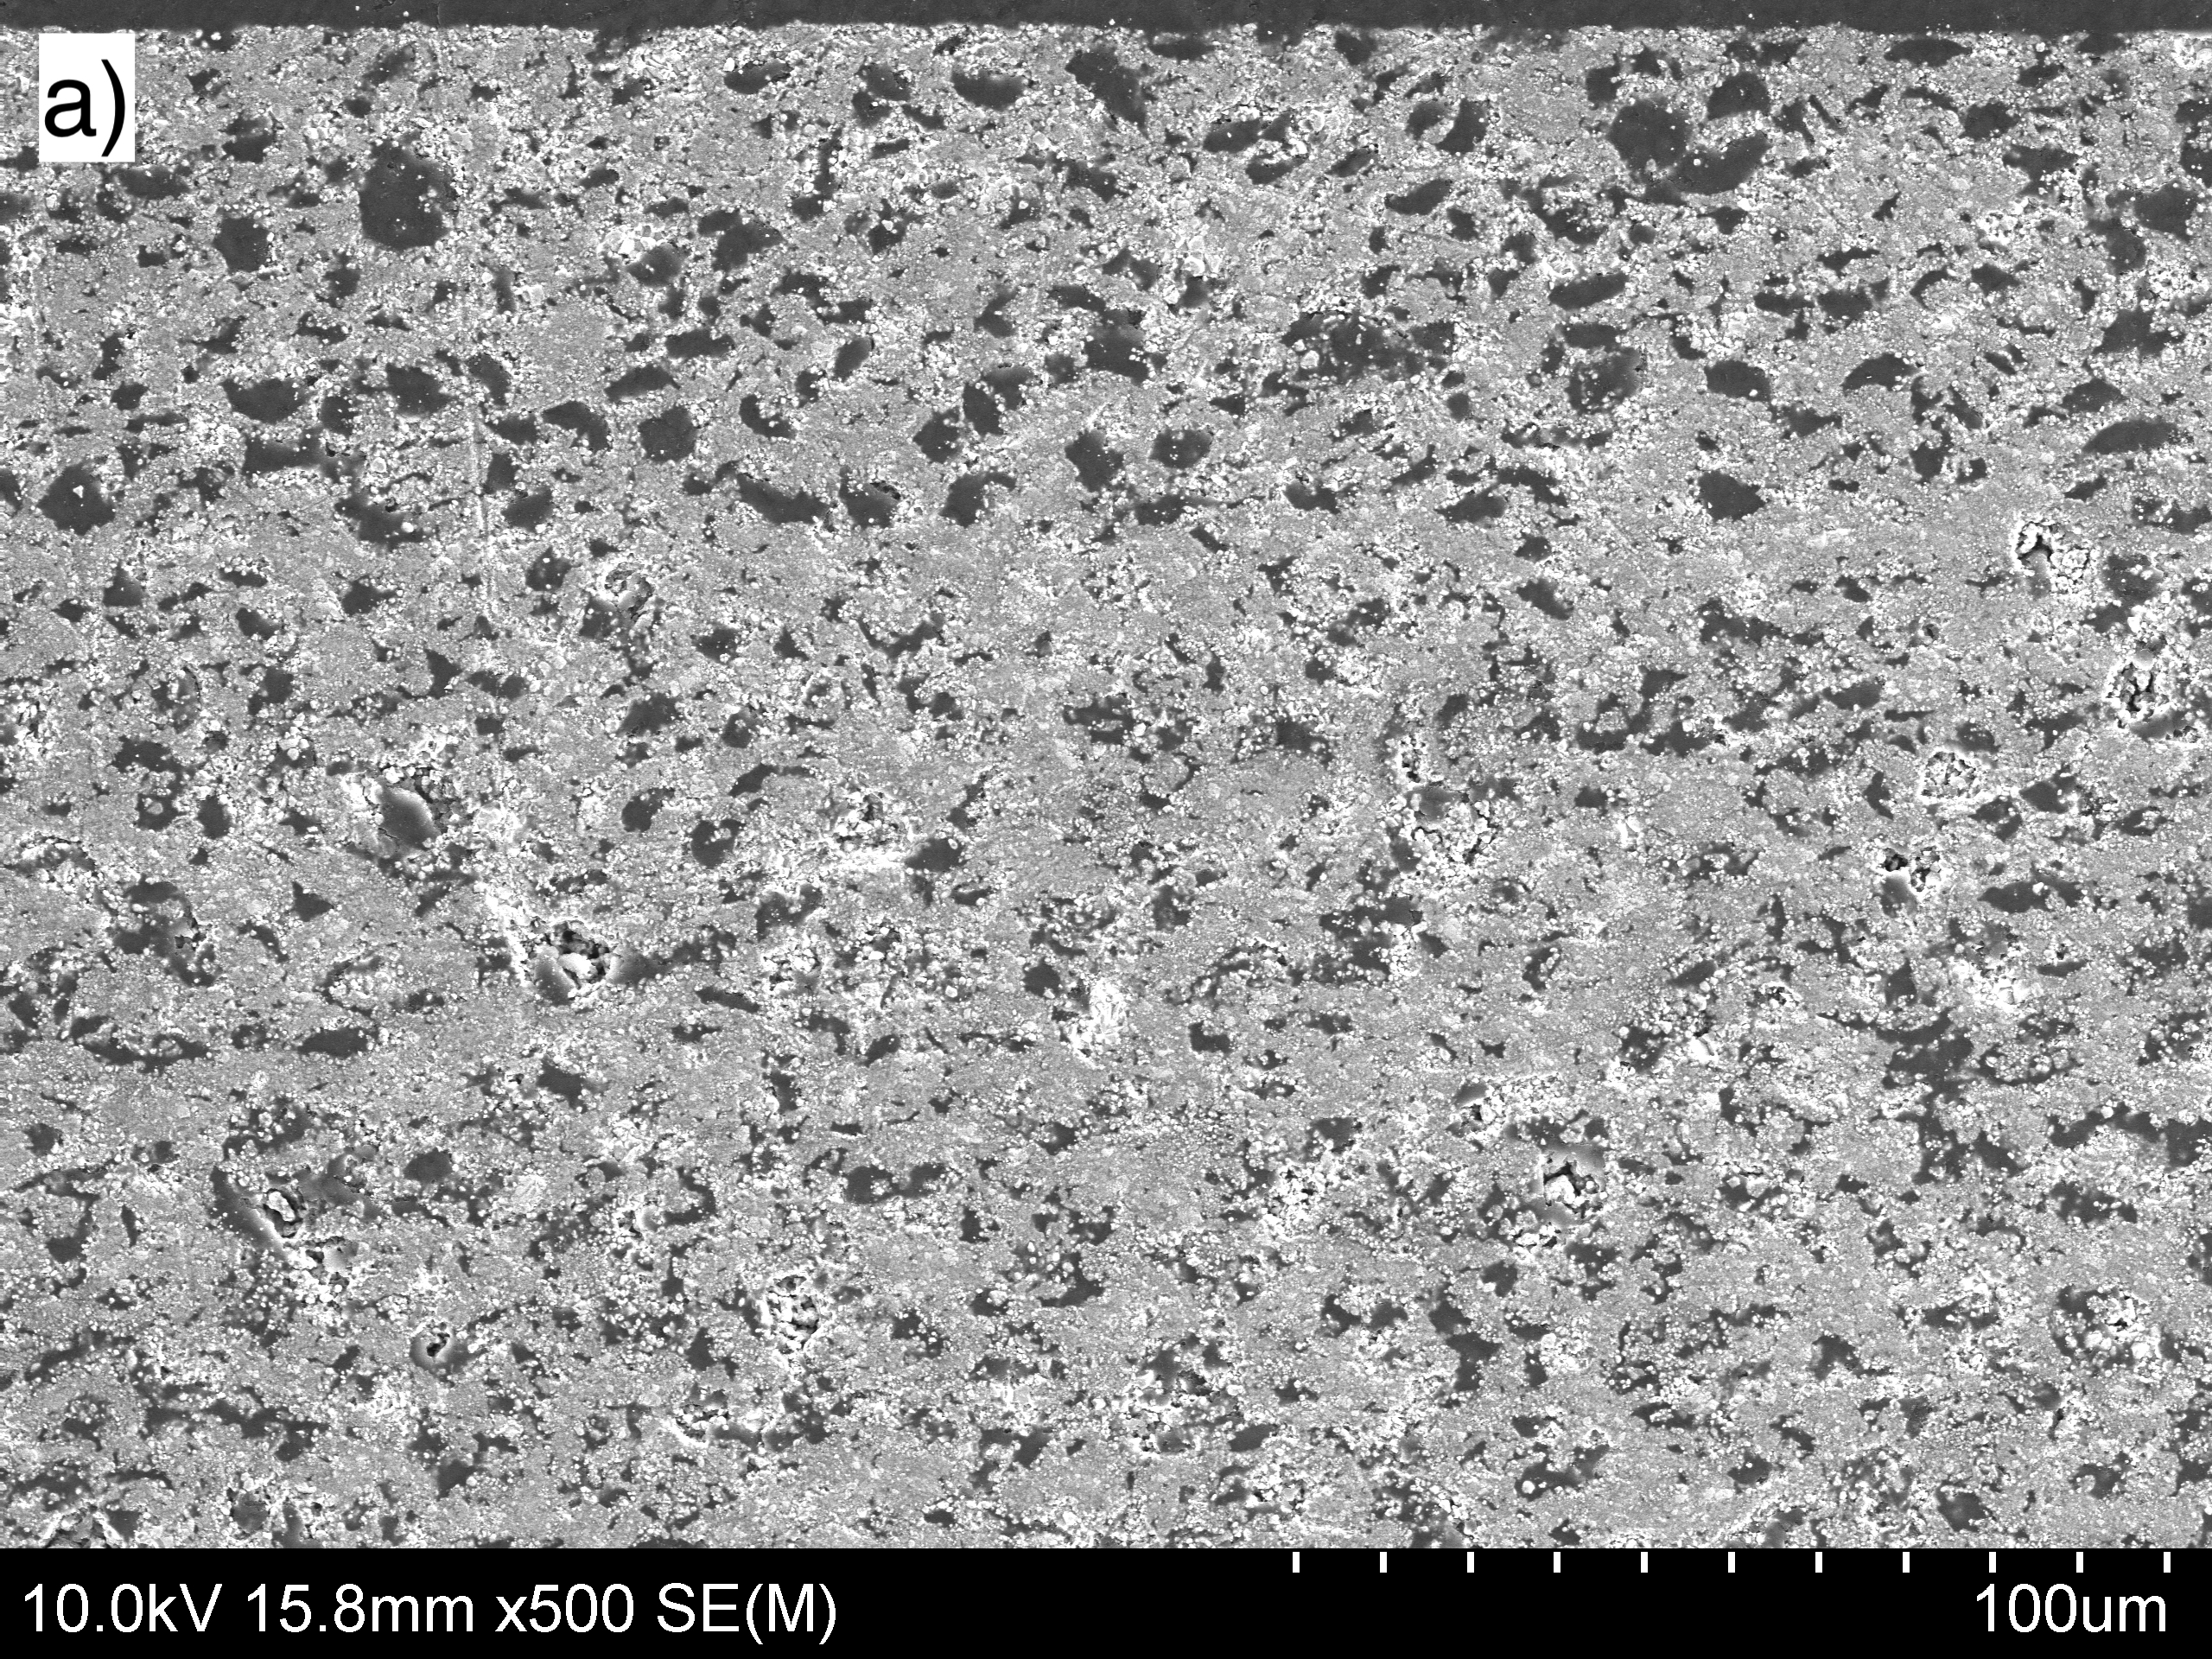
\includegraphics[width=0.75\textwidth]{0cycles.jpg}
          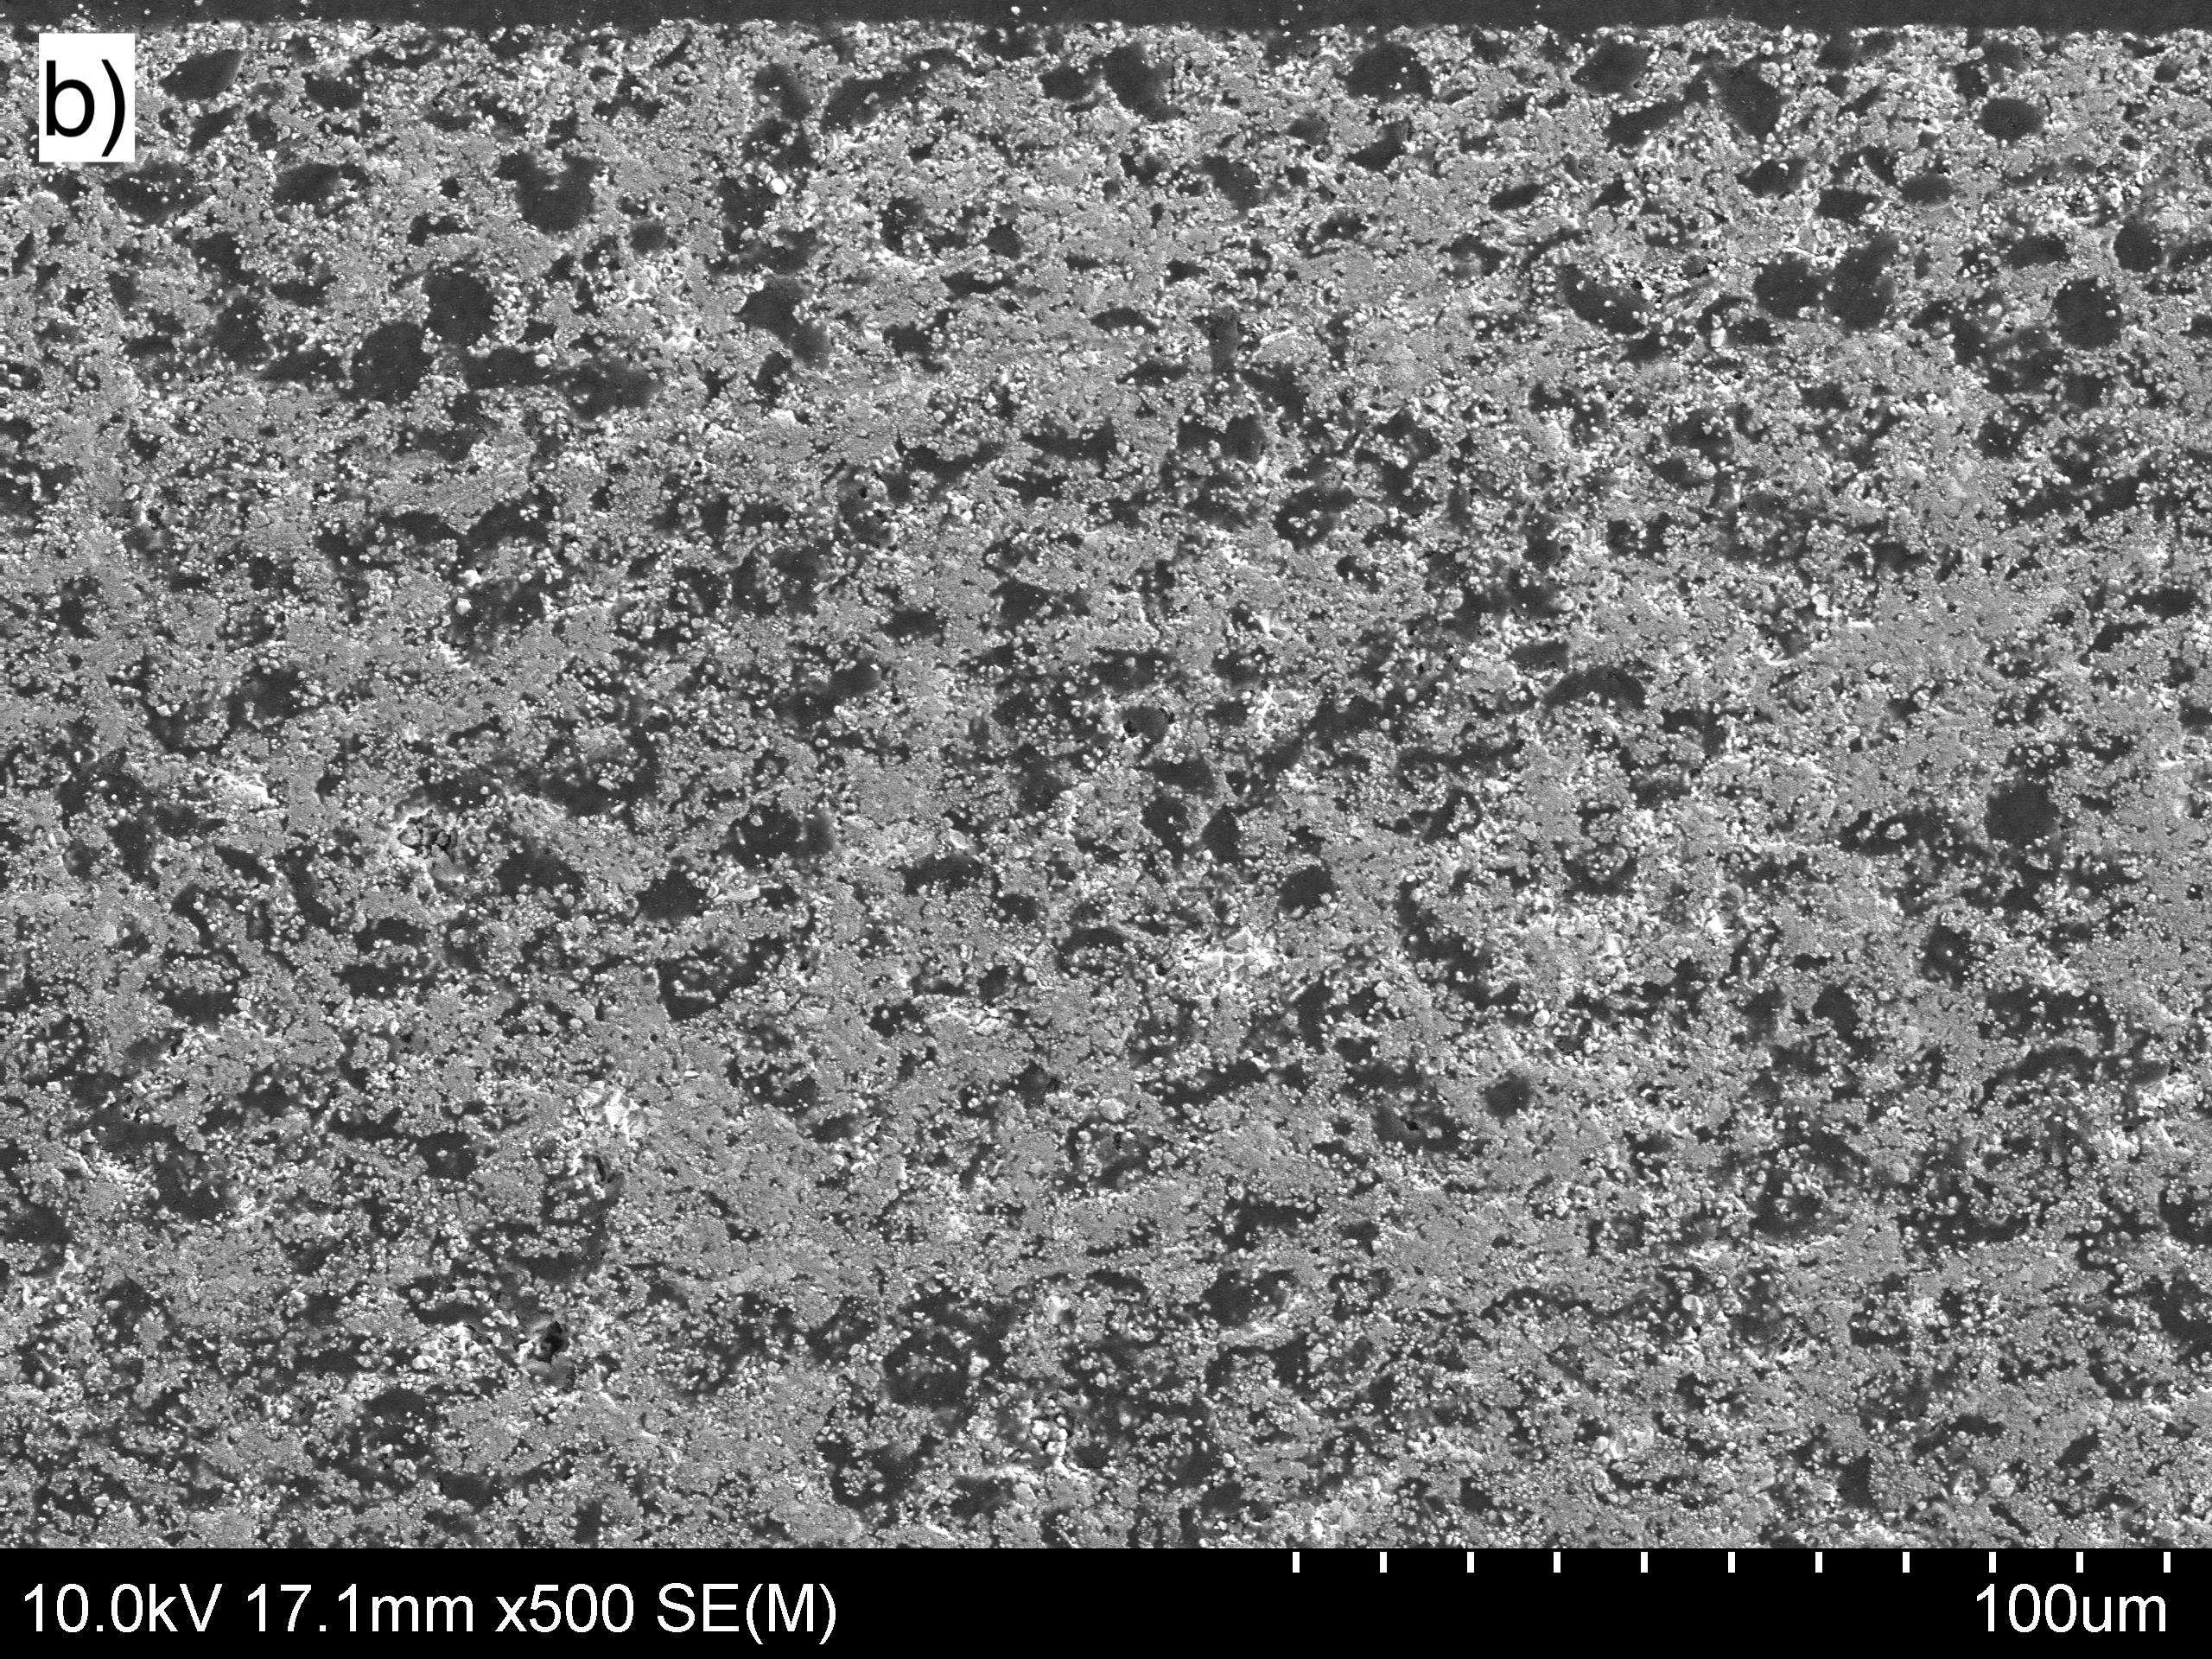
\includegraphics[width=0.75\textwidth]{10cycles.jpg}
          \caption{Scanning electron microscope images of epoxy-filled and polished SFCM-GDC \gls{asl}  cross sections tested a) before any cycling, b) after 10 cycles between 10\% H\textsubscript{2} and N\textsubscript{2}}
          \label{fig:cycledSEM}
        \end{figure}

\section{Conclusions}
    In this work, the mechanical properties of SFCM and SFCM-GDC structures are characterized as the environment is changed from ambient to the working conditions of SOFCs and with redox cycling.
    The electrical conductivity of SFCM-GDC is stable up to 19 cycles due to the reversibility and phase stability of SFCM-GDC in the environment range.
    The fracture toughness of SFCM was found to be \SI[separate-uncertainty = true]{0.124 +- 0.023}{\mega\pascal\sqrt{m}} at room temperature and increases with temperature, due to relaxation of residual stresses.
    The flexural strength of SFCM-GDC/GDC half-cells increases by 23.9\% upon heating from room temperature to \SI{600}{\celsius}.
    This is due to thermal expansion pushing cracks closed during heating, requiring additional stress to propagate surface cracks and the increase in fracture toughness.
    Once exposed to reducing conditions, the flexural strength decreases by 29.4\% of the original strength, as impurities reduce and SFCM and GDC generate oxygen vacancies.
    Reduction was shown to increase the size and variability of the distribution of flaws which lead to failure.
    Redox cycling led to the uniform increase in critical flaw size and changed the fine microstructural porosity, decreasing strength from \SI{34.3}{\mega\pascal} to \SI{22.4}{\mega\pascal}.

    These findings show that SFCM, when combined with GDC, make a suitable anode material for SOFCs.
    SFCM-GDC is a stable material system, both in terms of conductivity and mechanically, with redox cycling.
    Reduction does increase the likelihood of failure by decreasing characteristic strength and the distribution of flaws, but repeated cycling only decreases characteristic strength and does not change the Weibull modulus.
